\section{Results\label{sec:results}}
This section shows performance for the proposed bus charging algorithm and contains three subsections. Section \ref{sec:results:prior} compares the proposed method with a previously published algorithm \cite{He_2019_Fast}. Section \ref{sec:results:time} discusses the difference in computation time between prior work and the current method.
\par The comparisons in this section consider a 5 bus, 5 charger scenario with a charge rate of 300 kW. Each solution is expressed in terms of a MILP and solved up to a 2\% gap using Gurobi \cite{gurobi}, unless otherwise specified. The uncontrolled loads from Section \ref{sec:uncontrolled} are represented with a scaled version of historical data from the Trax Power Substation at UTA. The scaling served to increase the difficulty of the charging problem and better illustrates the capabilities of the proposed algorithm. 

\subsection{Cost Comparison with Prior Work\label{sec:results:prior}} 
This section compares the monthly cost of energy for the proposed method with two other methods. The first method is a baseline algorithm that simulates how bus drivers at the Utah Transit Authority (UTA) in Salt Lake City (SLC) charge by default. The second method comes from \cite{He_2019_Fast}, which was selected because it is very similar to the proposed algorithm. The charge plan for all three methods is computed using mixed integer linear programs as described below.  
\par Conversations with bus drivers at the UTA in SLC have shown that bus drivers generally top off their batteries whenever a charger is available. In essence, the bus drivers are solving a maximization problem by default as they maximize the number of charge sessions in a day. Hence, the baseline algorithm follows the constraints in Eqn. \eqref{eqn:objective:final} but incentivizes buses to charge as frequently as possible. Let $v_{\sigma}^{ijk}$ be the value of the objective function $v$ at the index corresponding to $\sigma_{ijk}$ from section \ref{sec:formulation:constraint}. By letting $v^{ijk}_{\sigma} = -1, \ \forall i,j,k$ and zero otherwise, the baseline method effectively maximizes the number of times a bus can charge.  
 All methods are evaluated according to the rate schedule in \cite{rocky_mountain_power_rocky_2021}. 
 \par A comparison of all three algorithms is given in Fig. \ref{fig:costComparison}. Note how the cost of energy is generally the same for each algorithm and that the primary differences in cost come from the on-peak and facilities power charges, illustrating the need to minimize peak average power. To understand the difference in power management between the baseline and the proposed method, refer to Fig. \ref{fig:totalPower}. Note how the power for the proposed method (blue line) is almost completely flat, indicating a steady power use. In comparison, the baseline algorithm (red line) is less steady and includes periods of high power use, which leads to the increased power charges in Fig. \ref{fig:costComparison}.
 \par A similar phenomena is observed when comparing the proposed method to \cite{He_2019_Fast}. Fig. \ref{fig:powerPlot} compares the average power for the proposed algorithm and \cite{He_2019_Fast}.  Note how the proposed algorithm shifts the timing of charging events to produce a charge profile (blue line) that is complementary to the uncontrolled load (tan line).  When the uncontrolled load increases the bus load decreases, yielding a flat overall load profile (not shown), whereas the load profile from \cite{He_2019_Fast} (red line) shifts charging events to minimize charging during on-peak periods only, but ignores uncontrolled loads. The ability of the proposed method to produce a consistent load profile improves upon \cite{He_2019_Fast} because it accounts for the effects of uncontrolled loads and the costs of average power.  
\begin{figure}
	\centering
	\makeComparisonBarChartThree{media/7_objective/costComparison5Bus5ChargersAugmented.csv}{Cost (Dollars)}{Baseline}{He et al.}{Proposed}
	\caption{Cost comparison with prior work}
	\label{fig:costComparison}
\end{figure} 


\begin{figure*}
	\centering
	\makeComparisonTotalPowerPTwo{\rootdirectorytwo/media/7_objective/optimized5Bus5ChargerAugmentedTotalPowerPlot.csv}{\rootdirectorytwo/media/7_objective/baseline5Bus5ChargerAugmentedTotalPowerPlot.csv}{15-Minute Average Power (kW)}{Proposed}{Baseline}
	\caption{15-Minute average power for one day}
	\label{fig:totalPower}
\end{figure*}


\begin{figure*}
	\centering
	\makeComparisonPowerPTwo{\rootdirectorytwo/media/7_objective/optimized5Bus5ChargerAugmentedPowerPlot.csv}{\rootdirectorytwo/media/7_objective/HeEtAl5Bus5ChargerAugmentedPowerPlot.csv}{15-Minute Average Power (kW)}{Proposed}{He et al.}
	\caption{Comparison between uncontrolled and bus loads}
	\label{fig:powerPlot}
\end{figure*}

 
\subsection{Scalability\label{sec:results:scalability}}
\begin{figure}
	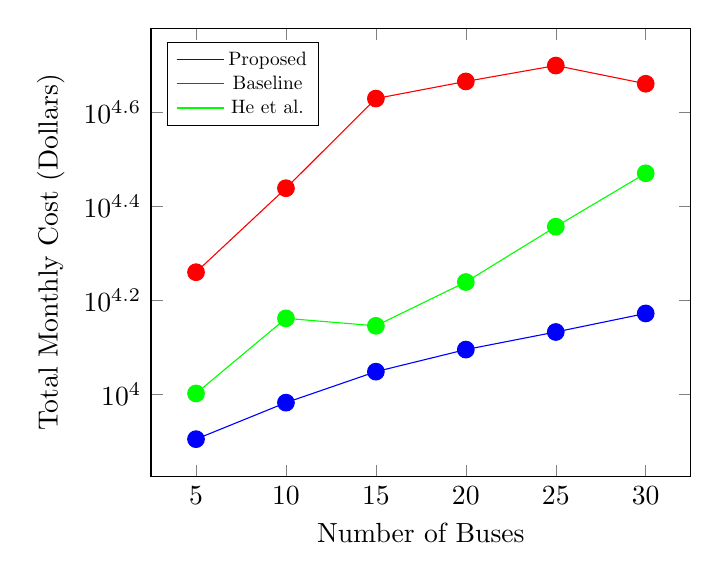
\begin{tikzpicture}
		\begin{axis}[xlabel=Number of Buses, ymode=log, ylabel=Total Monthly Cost (Dollars), legend pos=north west, legend style={nodes={scale=0.7}}]
			\addplot[blue] coordinates {
				(5,  8021.04 )
				(10, 9593.22 )
				(15, 11168.10)
				(20, 12445.52)
				(25, 13566.28)
				(30, 14857.82)}; 
			\addplot[red] coordinates{
				(5,  18190.02)
				(10, 27455.96)
				(15, 42618.54)
				(20, 46349.84)
				(25, 50101.33)
				(30, 45824.02)}; 
			\addplot[green] coordinates{
				(5,  10035.42)
				(10, 14505.31)
				(15, 13983.69)
				(20, 17333.25)
				(25, 22734.91)
				(30, 29543.78)
				};
			\addplot[blue, only marks, mark size=3pt] coordinates {
				(5,  8021.04 )
				(10, 9593.22 )
				(15, 11168.10)
				(20, 12445.52)
				(25, 13566.28)
				(30, 14857.82)}; 
			\addplot[red, only marks, mark size=3pt] coordinates{
				(5,  18190.02)
				(10, 27455.96)
				(15, 42618.54)
				(20, 46349.84)
				(25, 50101.33)
				(30, 45824.02)};
			\addplot[green, only marks, mark size=3pt] coordinates{
				(5,  10035.42)
				(10, 14505.31)
				(15, 13983.69)
				(20, 17333.25)
				(25, 22734.91)
				(30, 29543.78)
				};
			\legend{Proposed, Baseline, He et al.}
		\end{axis}
	\end{tikzpicture}
	\caption{Monthly Cost with 5 Chargers}
	\label{fig:scalabilityCost}
\end{figure}



\begin{figure}
	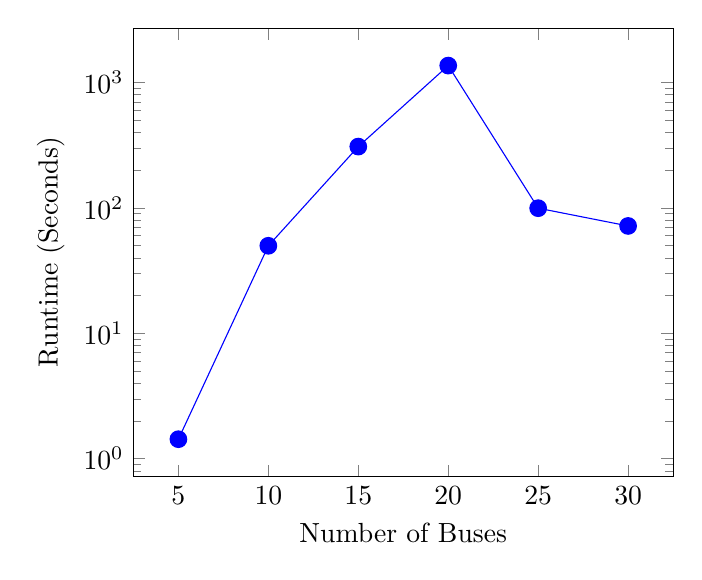
\begin{tikzpicture}
		\begin{axis}[xlabel=Number of Buses, ymode=log, ylabel=Runtime (Seconds)]
			\addplot[blue] coordinates {
				(5,  1.43  )
				(10, 49.92 )
				(15, 308.80)
				(20, 1367.0)
				(25, 99.59 )
				(30, 71.86 )};
			\addplot[blue, only marks, mark size=3pt] coordinates {
				(5,  1.43  )
				(10, 49.92 )
				(15, 308.80)
				(20, 1367.0)
				(25, 99.59 )
				(30, 71.86 )}; 
		\end{axis}
	\end{tikzpicture}
	\caption{Runtime with 5 Chargers at a 7\% Gap}
	\label{fig:scalabilityRuntime}
\end{figure}



In this section we discuss the limitations for scaling the proposed method with respect to the number of buses. Specifically, we desire to show that the proposed method both performs well with large numbers for buses and can be computed in a reasonable period of time. In Fig. \ref{fig:scalabilityCost}, we show how the cost increases with additional buses. Note how the monthly cost of power generally increases by approximately \$780 per bus, and that the relationship between cost and bus is linear. This indicates that for each additional bus in the fleet, the added expense comes from energy because the peak loads are initelligently managed. Additionally, the baseline algorithm which refuels buses whenever there is an opportunity reports significant cpst increases as the number of buses increase. It is interesting to note how the cost does taper as the bus-to-charger ratio increases, which is not unreasonable as the baseline method does not optimize with respect to cost. The differences between the proposed method and \cite{He_2019_Fast} continued to scale as well so the proposed outperformed both the baseline and the method given in \cite{He_2019_Fast} in scenarios where there were more buses. 
\par The results for Fig. \ref{fig:scalabilityRuntime} were obtained by optimizing the monthly cost of 5 to 30 buses up to a 7\% gap.  Note how the runtime increases significantly as the fleet size increases from 5 to 20 buses and then begins to decrease as the fleet size grows to 30 buses.  To understand this behavior, recall that the optimizer is essentially addressing two problems. The first problem is how to schedule charging sessions so that each bus leaves on time and carries sufficient charge. The second problem is to minimise the monthly cost of charging. When the fleet size is small, there are many different charging schedules that meet time and charge constraints and the optimizer has flexibility to select the schedule that minimizes cost. As fleet size increases, the complexity of the scheduling problem increases and this is manifest in increasing runtimes.  Past a certain point (above 20 buses in the given scenario) contention for time on the chargers increases and there are fewer charging schedules that meet time and charge constraints.  The optimizer has fewer options from which to choose (smaller feasible set) and the optimizer converges more quickly, reducing runtimes.
